\section{Pruebas de Funcionamiento}


    \subsection{Introducción}
        En esta sección se describen las pruebas realizadas para validar el funcionamiento del controlador de vuelo en conjunto. Primeramente se van a describir ciertas pruebas que se realizaron a cada sección de componentes, verificando su funcionamiento individual y la estabilidad del sistema bajo condiciones operativas.
    \subsection{Prueba de Almacenamiento de Datos}
        \vspace{5 px}
        Para este apartado de prueba de datos se utilizo el modulo de Almacenamiento de Datos que esta situado en la parte inferior del dispositivo tal y como se observa en la imagen , seguidamente se procedió a configurar la \textbf{ESP32-S3} para poder escribir y guardar datos en una unidad \textbf{microSD}. Para realizar esto, debemos recordar que la comunicación con el modulo de almacenamiento de datos se realiza mediante el protocolo \textbf{SPI} por lo que se debe instanciar los pines de \textbf{MISO, MOSI, SCK, CS} de este protocolo con los siguientes\textbf{GPIOS} :
        \vspace{5 px}
        \begin{lstlisting}[language=C++]
        #define MOSI_PIN 35
        #define SCK_PIN 36
        #define MISO_PIN 37
        #define CS_PIN 38
        \end{lstlisting}

        \vspace{5 px}

        Posteriormente, se procedió a realizar un script que fuera capaz de leer la cantidad de archivos en la unidad de almacenamiento y ponerle una cabecera de nombre que fuera \textbf{dataSaved\_n.csv} donde \textbf{n} es la cantidad de archivos que tiene la \textbf{microSD}, de tal forma que el nombre fuese único cada vez que se reinicia el dispositivo. Esto se realizo de esta forma para evitar estar sobrescribiendo información en un mismo archivo. Adicionalmente, la información que se va a guardar en la microSD, es la información crucial de todos los datos de vuelo que el UAV ha generado desde su puesta de operación hasta el momento en el que se recupere esta información. \\
        \vspace{10 px}
        Para ver la capacidad de recolección de datos del dispositivos y el tamaño del archivo generado .Se procedió a dejar simulando el dispositivo durante 3  horas y 20 minutos, generando un archivo CSV con un tamaño de 1,18 MB (1.245.184 bytes). El archivo contiene un total de 17.031 líneas de datos.


        Para estimar la capacidad de almacenamiento a largo plazo, realizamos una proyección utilizando una memoria de 64 GB. A continuación, se muestra el cálculo detallado:

        \vspace{5 px}
        \begin{itemize}
            \item Tamaño del archivo generado: 1,18 MB (1.245.184 bytes)
            \item Duración de la prueba: 3 horas y 20 minutos (3,33 horas)
            \item Número de líneas en el archivo: 17.031
        \end{itemize}
        \vspace{5 px}
        Para determinar cuántas horas de operación se pueden almacenar en una memoria de 64 GB (68.719.476.736 bytes), utilizamos la siguiente regla de tres:

        \begin{equation}
        \frac{1.245.184 \, \text{bytes}}{3,33 \, \text{horas}} = \frac{68.719.476.736 \, \text{bytes}}{x \, \text{horas}}
        \end{equation}

        Despejando \( x \):

        \begin{equation}
        x = \frac{68.719.476.736 \, \text{bytes} \times 3,33 \, \text{horas}}{1.245.184 \, \text{bytes}} = 183.816,34 \, \text{horas}
        \end{equation}

        Para convertir las horas de operación a años, usamos la relación de 1 año = 8.760 horas:

        \begin{equation}
        \frac{183.816,34 \, \text{horas}}{8.760 \, \text{horas/año}} = 20,99 \, \text{años}
        \end{equation}

        \vspace{5 px}
        Por lo tanto, se puede almacenar información en una memoria de 64 GB durante aproximadamente 183.816,34 horas o 20,99 años, considerando el ritmo de generación de datos y el tamaño de los archivos registrados en esta prueba.


    \subsection{Verificación de la lectura y escritura del valor de los servos con osciloscopio}

        Una vez configurado el apartado de lectura de los canales del transmisor \textbf{FLYSKY-I6}, se procedió a verificar que la lectura de los canales y la escritura de los valores \textbf{PWM} en la \textbf{PCA9685} se realizara correctamente. Para ello, se utilizó un osciloscopio para visualizar tanto la señal de entrada como la de salida, como se muestra en la figura (\ref{fig:pruebasPWM}).


        \begin{figure}[H]
            \centering
            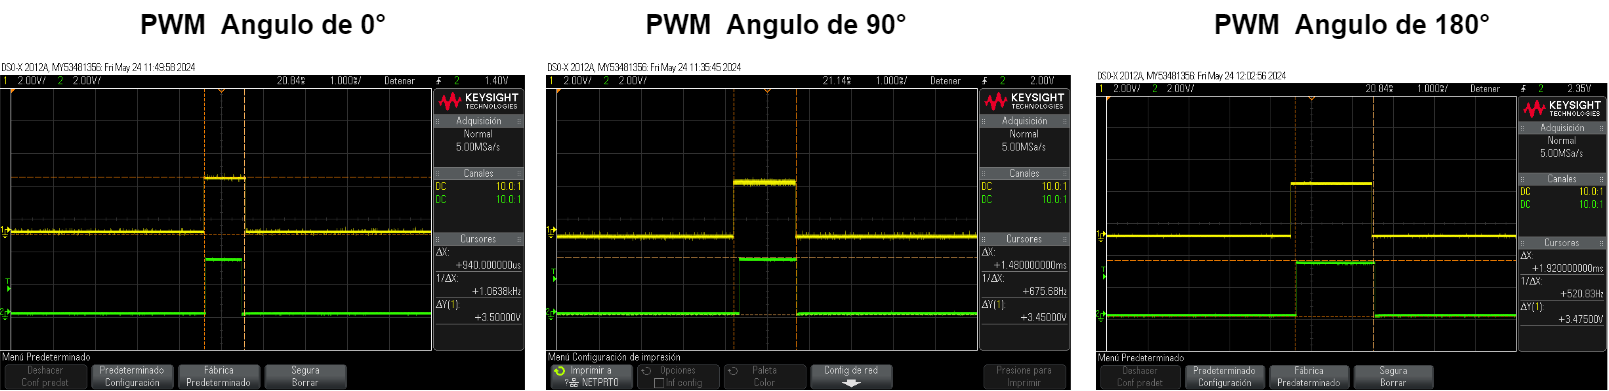
\includegraphics[width=7 in]{Imagenes/Pruebas/pwm canales.png}
            \caption{Pruebas de lectura y escritura valores PWM}
            \label{fig:pruebasPWM}
        \end{figure}

        La prueba del osciloscopio se realizó midiendo directamente en el pin de salida del receptor del canal 1 y en el pin de salida de la \textbf{PCA9685}. Los resultados mostraron que el cambio en la modulación por ancho de pulso (PWM) es proporcional al ángulo deseado, lo cual se puede evidenciar tanto en la lectura como en la escritura de los valores PWM.

        En la figura (\ref{fig:pruebasPWM}) se presentan tres capturas de pantalla del osciloscopio, que muestran las señales PWM correspondientes a ángulos de 0°, 90° y 180°. 

        \begin{itemize}
            \item En la primera imagen, se observa una señal PWM con un ángulo de 0°. La duración del pulso es de 940 $\mu$s, lo que indica la posición mínima posible.
            \item En la segunda imagen, la señal PWM corresponde a un ángulo de 90°. La duración del pulso es de 1.48 ms, indicando la posición por defecto o media del control.
            \item En la tercera imagen, la señal PWM corresponde a un ángulo de 180°. La duración del pulso es de 1.92 ms, indicando la posición máxima posible.
        \end{itemize}

        Adicionalmente, es importante señalar que en las imágenes la línea verde representa la señal del receptor, mientras que la línea amarilla representa la señal de la \textbf{PCA9685}. Estos resultados confirman que la modulación por ancho de pulso (PWM) cambia proporcionalmente con el ángulo deseado, garantizando un control preciso y predecible de los servomecanismos o actuadores conectados al sistema.
        \vspace{5 px}
    \subsection{Comparación de Controladores}
        \vspace{5 px}
        Para esta prueba, se compararon los valores de los ángulos de Roll y Pitch entre el controlador diseñado y un controlador comercial, el SpeedyBee V3 F405. Los dos controladores se situaron como se observa en la imagen y se configuraron los offsets iniciales para asegurar una medición precisa desde el mismo punto de referencia.
        \vspace{5 px}


        Para obtener los valores del controlador SpeedyBee, se utilizó la aplicación de Betaflight, la cual permite obtener los valores de Yaw, Pitch y Roll. Se contrastaron las mediciones cada diez grados de los ángulos y se puede observar en las imágenes que el comportamiento de ambos controladores es bastante similar.
        \vspace{5 px}
    \subsubsection{Descripción del SpeedyBee V3 F405}
        \vspace{5 px}
        El SpeedyBee V3 F405 es un controlador de vuelo comercial diseñado para drones. Este controlador es conocido por su estabilidad y precisión en la medición de ángulos, y es ampliamente utilizado en la comunidad de drones por su integración con la aplicación Betaflight, que facilita la configuración y obtención de datos de vuelo.
        \vspace{5 px}
        \begin{figure}[H]
            \centering
            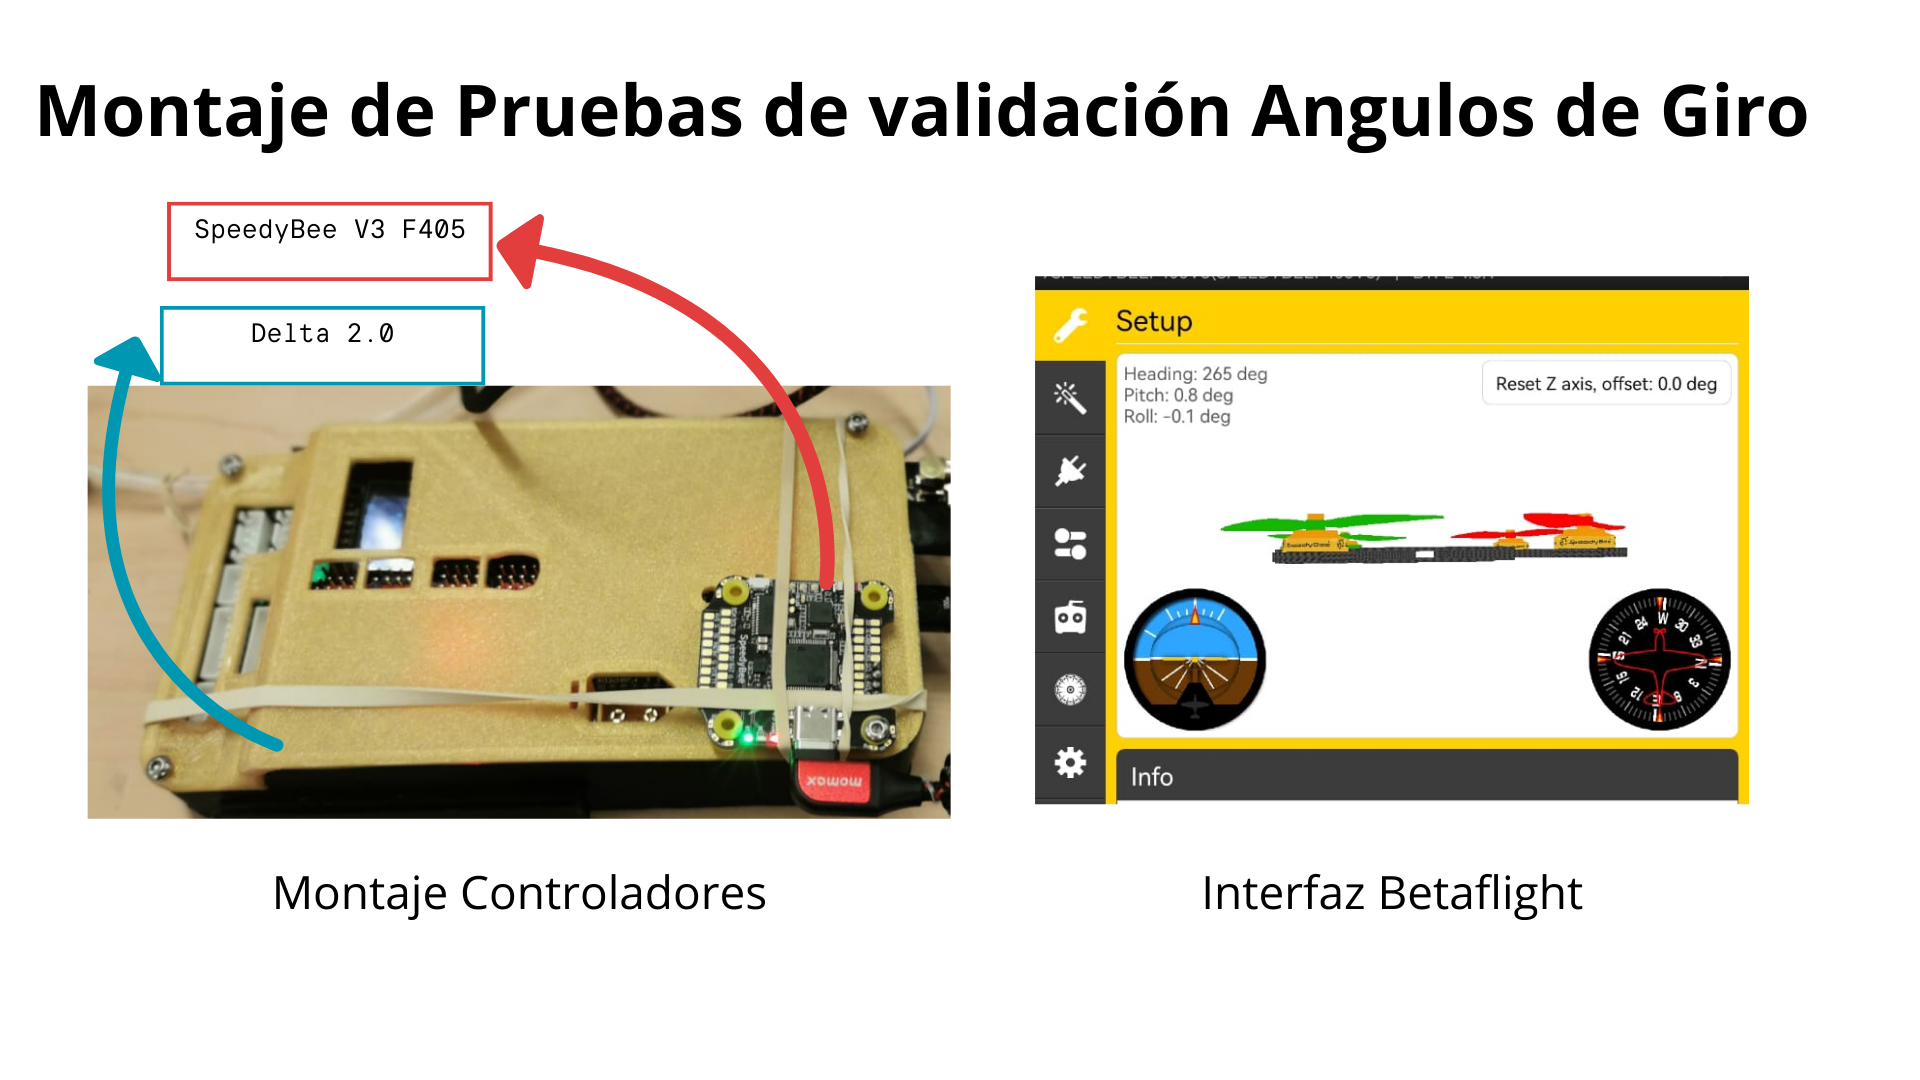
\includegraphics[width=\textwidth]{Imagenes/Pruebas/montajeControladores.png}
            \caption{Pruebas de validación y montaje controladores }
            \label{fig:pruebasPWM}
        \end{figure}



    \subsubsection{Resultados de la Prueba}



        \begin{table}[H] 
        \centering
        \caption{Toma de datos 1 y 2 para Roll}
        \resizebox{0.8\textwidth}{!}{

        \begin{tabular}{c|
        >{\columncolor[HTML]{C1F0C8}}c 
        >{\columncolor[HTML]{C1F0C8}}c 
        >{\columncolor[HTML]{C1F0C8}}c |
        >{\columncolor[HTML]{C0E6F5}}c 
        >{\columncolor[HTML]{C0E6F5}}c 
        >{\columncolor[HTML]{C0E6F5}}c |}
        \cline{2-7}
        \multicolumn{1}{l|}{}             & \multicolumn{3}{c|}{\cellcolor[HTML]{47D359}\textit{\textbf{Toma de datos 1}}}                                                                                                                                         & \multicolumn{3}{c|}{\cellcolor[HTML]{44B3E1}\textit{\textbf{Toma de datos 2}}}                                                                                                                                            \\ \hline
        \multicolumn{1}{|c|}{\textbf{X}}  & \multicolumn{1}{c|}{\cellcolor[HTML]{83E28E}\textit{\textbf{Roll SpeedyBee v3 f405}}} & \multicolumn{1}{c|}{\cellcolor[HTML]{83E28E}\textit{\textbf{Roll Delta}}} & \cellcolor[HTML]{83E28E}\textit{\textbf{\% Error}} & \multicolumn{1}{c|}{\cellcolor[HTML]{61CBF3}\textit{\textbf{Roll SpeedyBee v3 f405}}} & \multicolumn{1}{c|}{\cellcolor[HTML]{61CBF3}\textit{\textbf{Roll Delta  2}}} & \cellcolor[HTML]{61CBF3}\textit{\textbf{\% Error}} \\ \hline
        \multicolumn{1}{|c|}{\textbf{1}}  & \multicolumn{1}{c|}{\cellcolor[HTML]{C1F0C8}\textit{0}}                               & \multicolumn{1}{c|}{\cellcolor[HTML]{C1F0C8}\textit{0,44}}                & \textit{1\%}                                       & \multicolumn{1}{c|}{\cellcolor[HTML]{C0E6F5}\textit{0}}                               & \multicolumn{1}{c|}{\cellcolor[HTML]{C0E6F5}\textit{0}}                      & \textit{0}                                         \\ \hline
        \multicolumn{1}{|c|}{\textbf{2}}  & \multicolumn{1}{c|}{\cellcolor[HTML]{C1F0C8}\textit{10,3}}                            & \multicolumn{1}{c|}{\cellcolor[HTML]{C1F0C8}\textit{10,44}}               & \textit{1\%}                                       & \multicolumn{1}{c|}{\cellcolor[HTML]{C0E6F5}\textit{10,1}}                            & \multicolumn{1}{c|}{\cellcolor[HTML]{C0E6F5}\textit{10,38}}                  & \textit{3\%}                                       \\ \hline
        \multicolumn{1}{|c|}{\textbf{3}}  & \multicolumn{1}{c|}{\cellcolor[HTML]{C1F0C8}\textit{20,6}}                            & \multicolumn{1}{c|}{\cellcolor[HTML]{C1F0C8}\textit{20,2}}                & \textit{2\%}                                       & \multicolumn{1}{c|}{\cellcolor[HTML]{C0E6F5}\textit{19,5}}                            & \multicolumn{1}{c|}{\cellcolor[HTML]{C0E6F5}\textit{20,12}}                  & \textit{3\%}                                       \\ \hline
        \multicolumn{1}{|c|}{\textbf{4}}  & \multicolumn{1}{c|}{\cellcolor[HTML]{C1F0C8}\textit{31,2}}                            & \multicolumn{1}{c|}{\cellcolor[HTML]{C1F0C8}\textit{30,62}}               & \textit{2\%}                                       & \multicolumn{1}{c|}{\cellcolor[HTML]{C0E6F5}\textit{30,7}}                            & \multicolumn{1}{c|}{\cellcolor[HTML]{C0E6F5}\textit{30,69}}                  & \textit{0\%}                                       \\ \hline
        \multicolumn{1}{|c|}{\textbf{5}}  & \multicolumn{1}{c|}{\cellcolor[HTML]{C1F0C8}\textit{41,7}}                            & \multicolumn{1}{c|}{\cellcolor[HTML]{C1F0C8}\textit{40,19}}               & \textit{4\%}                                       & \multicolumn{1}{c|}{\cellcolor[HTML]{C0E6F5}\textit{40,8}}                            & \multicolumn{1}{c|}{\cellcolor[HTML]{C0E6F5}\textit{40,38}}                  & \textit{1\%}                                       \\ \hline
        \multicolumn{1}{|c|}{\textbf{6}}  & \multicolumn{1}{c|}{\cellcolor[HTML]{C1F0C8}\textit{52,1}}                            & \multicolumn{1}{c|}{\cellcolor[HTML]{C1F0C8}\textit{50,63}}               & \textit{3\%}                                       & \multicolumn{1}{c|}{\cellcolor[HTML]{C0E6F5}\textit{52}}                              & \multicolumn{1}{c|}{\cellcolor[HTML]{C0E6F5}\textit{50,25}}                  & \textit{3\%}                                       \\ \hline
        \multicolumn{1}{|c|}{\textbf{7}}  & \multicolumn{1}{c|}{\cellcolor[HTML]{C1F0C8}\textit{63,2}}                            & \multicolumn{1}{c|}{\cellcolor[HTML]{C1F0C8}\textit{60,56}}               & \textit{4\%}                                       & \multicolumn{1}{c|}{\cellcolor[HTML]{C0E6F5}\textit{61,3}}                            & \multicolumn{1}{c|}{\cellcolor[HTML]{C0E6F5}\textit{60,63}}                  & \textit{1\%}                                       \\ \hline
        \multicolumn{1}{|c|}{\textbf{8}}  & \multicolumn{1}{c|}{\cellcolor[HTML]{C1F0C8}\textit{72,8}}                            & \multicolumn{1}{c|}{\cellcolor[HTML]{C1F0C8}\textit{70,5}}                & \textit{3\%}                                       & \multicolumn{1}{c|}{\cellcolor[HTML]{C0E6F5}\textit{73,2}}                            & \multicolumn{1}{c|}{\cellcolor[HTML]{C0E6F5}\textit{70,12}}                  & \textit{4\%}                                       \\ \hline
        \multicolumn{1}{|c|}{\textbf{9}}  & \multicolumn{1}{c|}{\cellcolor[HTML]{C1F0C8}\textit{83,1}}                            & \multicolumn{1}{c|}{\cellcolor[HTML]{C1F0C8}\textit{80,56}}               & \textit{3\%}                                       & \multicolumn{1}{c|}{\cellcolor[HTML]{C0E6F5}\textit{84,2}}                            & \multicolumn{1}{c|}{\cellcolor[HTML]{C0E6F5}\textit{80,44}}                  & \textit{4\%}                                       \\ \hline
        \multicolumn{1}{|c|}{\textbf{10}} & \multicolumn{1}{c|}{\cellcolor[HTML]{C1F0C8}\textit{86,5}}                            & \multicolumn{1}{c|}{\cellcolor[HTML]{C1F0C8}\textit{87,1}}                & \textit{1\%}                                       & \multicolumn{1}{c|}{\cellcolor[HTML]{C0E6F5}\textit{92,9}}                            & \multicolumn{1}{c|}{\cellcolor[HTML]{C0E6F5}\textit{88,44}}                  & \textit{5\%}                                       \\ \hline
        \multicolumn{1}{|c|}{\textbf{11}} & \multicolumn{1}{c|}{\cellcolor[HTML]{C1F0C8}\textit{-8,7}}                            & \multicolumn{1}{c|}{\cellcolor[HTML]{C1F0C8}\textit{-10,38}}              & \textit{19\%}                                      & \multicolumn{1}{c|}{\cellcolor[HTML]{C0E6F5}\textit{-9,6}}                            & \multicolumn{1}{c|}{\cellcolor[HTML]{C0E6F5}\textit{-10,56}}                 & \textit{10\%}                                      \\ \hline
        \multicolumn{1}{|c|}{\textbf{12}} & \multicolumn{1}{c|}{\cellcolor[HTML]{C1F0C8}\textit{-19,8}}                           & \multicolumn{1}{c|}{\cellcolor[HTML]{C1F0C8}\textit{-20,31}}              & \textit{3\%}                                       & \multicolumn{1}{c|}{\cellcolor[HTML]{C0E6F5}\textit{-19,1}}                           & \multicolumn{1}{c|}{\cellcolor[HTML]{C0E6F5}\textit{-20,25}}                 & \textit{6\%}                                       \\ \hline
        \multicolumn{1}{|c|}{\textbf{13}} & \multicolumn{1}{c|}{\cellcolor[HTML]{C1F0C8}\textit{-30}}                             & \multicolumn{1}{c|}{\cellcolor[HTML]{C1F0C8}\textit{-30,19}}              & \textit{1\%}                                       & \multicolumn{1}{c|}{\cellcolor[HTML]{C0E6F5}\textit{-29,4}}                           & \multicolumn{1}{c|}{\cellcolor[HTML]{C0E6F5}\textit{-30,25}}                 & \textit{3\%}                                       \\ \hline
        \multicolumn{1}{|c|}{\textbf{14}} & \multicolumn{1}{c|}{\cellcolor[HTML]{C1F0C8}\textit{-40,7}}                           & \multicolumn{1}{c|}{\cellcolor[HTML]{C1F0C8}\textit{-39,1}}               & \textit{4\%}                                       & \multicolumn{1}{c|}{\cellcolor[HTML]{C0E6F5}\textit{-39,1}}                           & \multicolumn{1}{c|}{\cellcolor[HTML]{C0E6F5}\textit{-40,13}}                 & \textit{3\%}                                       \\ \hline
        \multicolumn{1}{|c|}{\textbf{15}} & \multicolumn{1}{c|}{\cellcolor[HTML]{C1F0C8}\textit{-50,9}}                           & \multicolumn{1}{c|}{\cellcolor[HTML]{C1F0C8}\textit{-50,63}}              & \textit{1\%}                                       & \multicolumn{1}{c|}{\cellcolor[HTML]{C0E6F5}\textit{-49,2}}                           & \multicolumn{1}{c|}{\cellcolor[HTML]{C0E6F5}\textit{-50,88}}                 & \textit{3\%}                                       \\ \hline
        \multicolumn{1}{|c|}{\textbf{16}} & \multicolumn{1}{c|}{\cellcolor[HTML]{C1F0C8}\textit{-59,8}}                           & \multicolumn{1}{c|}{\cellcolor[HTML]{C1F0C8}\textit{-60,25}}              & \textit{1\%}                                       & \multicolumn{1}{c|}{\cellcolor[HTML]{C0E6F5}\textit{-59,5}}                           & \multicolumn{1}{c|}{\cellcolor[HTML]{C0E6F5}\textit{-60,75}}                 & \textit{2\%}                                       \\ \hline
        \multicolumn{1}{|c|}{\textbf{17}} & \multicolumn{1}{c|}{\cellcolor[HTML]{C1F0C8}\textit{-69,7}}                           & \multicolumn{1}{c|}{\cellcolor[HTML]{C1F0C8}\textit{-70,37}}              & \textit{1\%}                                       & \multicolumn{1}{c|}{\cellcolor[HTML]{C0E6F5}\textit{-67,8}}                           & \multicolumn{1}{c|}{\cellcolor[HTML]{C0E6F5}\textit{-70,19}}                 & \textit{4\%}                                       \\ \hline
        \multicolumn{1}{|c|}{\textbf{18}} & \multicolumn{1}{c|}{\cellcolor[HTML]{C1F0C8}\textit{-80,1}}                           & \multicolumn{1}{c|}{\cellcolor[HTML]{C1F0C8}\textit{-80,69}}              & \textit{1\%}                                       & \multicolumn{1}{c|}{\cellcolor[HTML]{C0E6F5}\textit{-77,9}}                           & \multicolumn{1}{c|}{\cellcolor[HTML]{C0E6F5}\textit{-80,81}}                 & \textit{4\%}                                       \\ \hline
        \multicolumn{1}{|c|}{\textbf{19}} & \multicolumn{1}{c|}{\cellcolor[HTML]{C1F0C8}\textit{-89,2}}                           & \multicolumn{1}{c|}{\cellcolor[HTML]{C1F0C8}\textit{-90,06}}              & \textit{1\%}                                       & \multicolumn{1}{c|}{\cellcolor[HTML]{C0E6F5}\textit{-87,3}}                           & \multicolumn{1}{c|}{\cellcolor[HTML]{C0E6F5}\textit{-90,06}}                 & \textit{3\%}                                       \\ \hline
        \end{tabular}
        }

        \end{table}



        % Please add the following required packages to your document preamble:
        % \usepackage[table,xcdraw]{xcolor}
        % Beamer presentation requires \usepackage{colortbl} instead of \usepackage[table,xcdraw]{xcolor}
        \begin{table}[H] 

        \centering
        \caption{Toma de datos 1 y 2 para Pitch}
        \resizebox{0.8\textwidth}{!}{

        \begin{tabular}{c|
        >{\columncolor[HTML]{F2CEEF}}c 
        >{\columncolor[HTML]{F2CEEF}}c 
        >{\columncolor[HTML]{F2CEEF}}c |
        >{\columncolor[HTML]{CCCCFF}}c 
        >{\columncolor[HTML]{CCCCFF}}c 
        >{\columncolor[HTML]{CCCCFF}}c |}
        \cline{2-7}
        \multicolumn{1}{l|}{}             & \multicolumn{3}{c|}{\cellcolor[HTML]{D86DCD}\textbf{Toma de datos 1}}                                                                                                                          & \multicolumn{3}{c|}{\cellcolor[HTML]{6666FF}\textbf{Toma de datos 2}}                                                                                                                            \\ \hline
        \multicolumn{1}{|c|}{\textbf{X}}  & \multicolumn{1}{c|}{\cellcolor[HTML]{E49EDD}\textbf{Pitch  SpeedyBee v3 f405}} & \multicolumn{1}{c|}{\cellcolor[HTML]{E49EDD}\textbf{Pitch Delta}} & \cellcolor[HTML]{E49EDD}\textbf{\% Error} & \multicolumn{1}{c|}{\cellcolor[HTML]{9999FF}\textbf{Pitch  SpeedyBee v3 f405}} & \multicolumn{1}{c|}{\cellcolor[HTML]{9999FF}\textbf{Pitch Delta 2}} & \cellcolor[HTML]{9999FF}\textbf{\% Error} \\ \hline
        \multicolumn{1}{|c|}{\textbf{1}}  & \multicolumn{1}{c|}{\cellcolor[HTML]{F2CEEF}0}                                 & \multicolumn{1}{c|}{\cellcolor[HTML]{F2CEEF}-0,44}                & 1\%                                       & \multicolumn{1}{c|}{\cellcolor[HTML]{CCCCFF}0,1}                               & \multicolumn{1}{c|}{\cellcolor[HTML]{CCCCFF}0,94}                   & 0\%                                       \\ \hline
        \multicolumn{1}{|c|}{\textbf{2}}  & \multicolumn{1}{c|}{\cellcolor[HTML]{F2CEEF}10,8}                              & \multicolumn{1}{c|}{\cellcolor[HTML]{F2CEEF}10,6}                 & 2\%                                       & \multicolumn{1}{c|}{\cellcolor[HTML]{CCCCFF}10,8}                              & \multicolumn{1}{c|}{\cellcolor[HTML]{CCCCFF}10,44}                  & 3\%                                       \\ \hline
        \multicolumn{1}{|c|}{\textbf{3}}  & \multicolumn{1}{c|}{\cellcolor[HTML]{F2CEEF}21,6}                              & \multicolumn{1}{c|}{\cellcolor[HTML]{F2CEEF}20,12}                & 7\%                                       & \multicolumn{1}{c|}{\cellcolor[HTML]{CCCCFF}19,8}                              & \multicolumn{1}{c|}{\cellcolor[HTML]{CCCCFF}20}                     & 1\%                                       \\ \hline
        \multicolumn{1}{|c|}{\textbf{4}}  & \multicolumn{1}{c|}{\cellcolor[HTML]{F2CEEF}31,9}                              & \multicolumn{1}{c|}{\cellcolor[HTML]{F2CEEF}30,44}                & 5\%                                       & \multicolumn{1}{c|}{\cellcolor[HTML]{CCCCFF}30,1}                              & \multicolumn{1}{c|}{\cellcolor[HTML]{CCCCFF}30,31}                  & 1\%                                       \\ \hline
        \multicolumn{1}{|c|}{\textbf{5}}  & \multicolumn{1}{c|}{\cellcolor[HTML]{F2CEEF}41,9}                              & \multicolumn{1}{c|}{\cellcolor[HTML]{F2CEEF}40,13}                & 4\%                                       & \multicolumn{1}{c|}{\cellcolor[HTML]{CCCCFF}40,8}                              & \multicolumn{1}{c|}{\cellcolor[HTML]{CCCCFF}40,63}                  & 0\%                                       \\ \hline
        \multicolumn{1}{|c|}{\textbf{6}}  & \multicolumn{1}{c|}{\cellcolor[HTML]{F2CEEF}53,2}                              & \multicolumn{1}{c|}{\cellcolor[HTML]{F2CEEF}50,63}                & 5\%                                       & \multicolumn{1}{c|}{\cellcolor[HTML]{CCCCFF}50,1}                              & \multicolumn{1}{c|}{\cellcolor[HTML]{CCCCFF}50,19}                  & 0\%                                       \\ \hline
        \multicolumn{1}{|c|}{\textbf{7}}  & \multicolumn{1}{c|}{\cellcolor[HTML]{F2CEEF}63,5}                              & \multicolumn{1}{c|}{\cellcolor[HTML]{F2CEEF}60,96}                & 4\%                                       & \multicolumn{1}{c|}{\cellcolor[HTML]{CCCCFF}60,9}                              & \multicolumn{1}{c|}{\cellcolor[HTML]{CCCCFF}60,19}                  & 1\%                                       \\ \hline
        \multicolumn{1}{|c|}{\textbf{8}}  & \multicolumn{1}{c|}{\cellcolor[HTML]{F2CEEF}73,3}                              & \multicolumn{1}{c|}{\cellcolor[HTML]{F2CEEF}70,75}                & 3\%                                       & \multicolumn{1}{c|}{\cellcolor[HTML]{CCCCFF}71,5}                              & \multicolumn{1}{c|}{\cellcolor[HTML]{CCCCFF}70,44}                  & 1\%                                       \\ \hline
        \multicolumn{1}{|c|}{\textbf{9}}  & \multicolumn{1}{c|}{\cellcolor[HTML]{F2CEEF}83,3}                              & \multicolumn{1}{c|}{\cellcolor[HTML]{F2CEEF}80,12}                & 4\%                                       & \multicolumn{1}{c|}{\cellcolor[HTML]{CCCCFF}82,5}                              & \multicolumn{1}{c|}{\cellcolor[HTML]{CCCCFF}80,37}                  & 3\%                                       \\ \hline
        \multicolumn{1}{|c|}{\textbf{10}} & \multicolumn{1}{c|}{\cellcolor[HTML]{F2CEEF}86,3}                              & \multicolumn{1}{c|}{\cellcolor[HTML]{F2CEEF}87,06}                & 1\%                                       & \multicolumn{1}{c|}{\cellcolor[HTML]{CCCCFF}87,5}                              & \multicolumn{1}{c|}{\cellcolor[HTML]{CCCCFF}88}                     & 1\%                                       \\ \hline
        \multicolumn{1}{|c|}{\textbf{11}} & \multicolumn{1}{c|}{\cellcolor[HTML]{F2CEEF}-9,6}                              & \multicolumn{1}{c|}{\cellcolor[HTML]{F2CEEF}-10,38}               & 8\%                                       & \multicolumn{1}{c|}{\cellcolor[HTML]{CCCCFF}-11,8}                             & \multicolumn{1}{c|}{\cellcolor[HTML]{CCCCFF}-10,13}                 & 14\%                                      \\ \hline
        \multicolumn{1}{|c|}{\textbf{12}} & \multicolumn{1}{c|}{\cellcolor[HTML]{F2CEEF}-20,5}                             & \multicolumn{1}{c|}{\cellcolor[HTML]{F2CEEF}-20,31}               & 1\%                                       & \multicolumn{1}{c|}{\cellcolor[HTML]{CCCCFF}-21,9}                             & \multicolumn{1}{c|}{\cellcolor[HTML]{CCCCFF}-20,81}                 & 5\%                                       \\ \hline
        \multicolumn{1}{|c|}{\textbf{13}} & \multicolumn{1}{c|}{\cellcolor[HTML]{F2CEEF}-29,6}                             & \multicolumn{1}{c|}{\cellcolor[HTML]{F2CEEF}-30,5}                & 3\%                                       & \multicolumn{1}{c|}{\cellcolor[HTML]{CCCCFF}-32,1}                             & \multicolumn{1}{c|}{\cellcolor[HTML]{CCCCFF}-30,44}                 & 5\%                                       \\ \hline
        \multicolumn{1}{|c|}{\textbf{14}} & \multicolumn{1}{c|}{\cellcolor[HTML]{F2CEEF}-40}                               & \multicolumn{1}{c|}{\cellcolor[HTML]{F2CEEF}-40,31}               & 1\%                                       & \multicolumn{1}{c|}{\cellcolor[HTML]{CCCCFF}-43,6}                             & \multicolumn{1}{c|}{\cellcolor[HTML]{CCCCFF}-40,75}                 & 7\%                                       \\ \hline
        \multicolumn{1}{|c|}{\textbf{15}} & \multicolumn{1}{c|}{\cellcolor[HTML]{F2CEEF}-49,2}                             & \multicolumn{1}{c|}{\cellcolor[HTML]{F2CEEF}-50,19}               & 2\%                                       & \multicolumn{1}{c|}{\cellcolor[HTML]{CCCCFF}-53,5}                             & \multicolumn{1}{c|}{\cellcolor[HTML]{CCCCFF}-50,44}                 & 6\%                                       \\ \hline
        \multicolumn{1}{|c|}{\textbf{16}} & \multicolumn{1}{c|}{\cellcolor[HTML]{F2CEEF}-58,3}                             & \multicolumn{1}{c|}{\cellcolor[HTML]{F2CEEF}-60,13}               & 3\%                                       & \multicolumn{1}{c|}{\cellcolor[HTML]{CCCCFF}-62,6}                             & \multicolumn{1}{c|}{\cellcolor[HTML]{CCCCFF}-60,75}                 & 3\%                                       \\ \hline
        \multicolumn{1}{|c|}{\textbf{17}} & \multicolumn{1}{c|}{\cellcolor[HTML]{F2CEEF}-69}                               & \multicolumn{1}{c|}{\cellcolor[HTML]{F2CEEF}-70,25}               & 2\%                                       & \multicolumn{1}{c|}{\cellcolor[HTML]{CCCCFF}-72,1}                             & \multicolumn{1}{c|}{\cellcolor[HTML]{CCCCFF}-70,5}                  & 2\%                                       \\ \hline
        \multicolumn{1}{|c|}{\textbf{18}} & \multicolumn{1}{c|}{\cellcolor[HTML]{F2CEEF}-78,9}                             & \multicolumn{1}{c|}{\cellcolor[HTML]{F2CEEF}-80,44}               & 2\%                                       & \multicolumn{1}{c|}{\cellcolor[HTML]{CCCCFF}-82,1}                             & \multicolumn{1}{c|}{\cellcolor[HTML]{CCCCFF}-80,62}                 & 2\%                                       \\ \hline
        \multicolumn{1}{|c|}{\textbf{19}} & \multicolumn{1}{c|}{\cellcolor[HTML]{F2CEEF}-87,5}                             & \multicolumn{1}{c|}{\cellcolor[HTML]{F2CEEF}-89,44}               & 2\%                                       & \multicolumn{1}{c|}{\cellcolor[HTML]{CCCCFF}-86,6}                             & \multicolumn{1}{c|}{\cellcolor[HTML]{CCCCFF}-87,19}                 & 1\%                                       \\ \hline
        \end{tabular}
        }
        \end{table}

        \subsubsection{Análisis de las Tablas}

            En las tablas de datos de Roll y Pitch, se observa que ambos controladores presentan comportamientos bastante similares. El error relativo entre las mediciones de los controladores Delta y SpeedyBee V3 F405 varía generalmente entre el 1\% y el 4\%. Sin embargo, hay excepciones notables, como cuando se miden ángulos cercanos a los -10°, tanto en Roll como en Pitch, donde el error puede llegar hasta el 19\%.

            \vspace{5px}
            Es importante destacar que existe cierta incertidumbre asociada a la forma en que se recopilaron los datos. Fijar los ángulos en diferentes grados puede introducir variaciones en las lecturas de ambos controladores debido a pequeñas discrepancias en la posición exacta y la respuesta de los sensores. Esto puede afectar la precisión de las mediciones comparadas.
            \vspace{5px}

        \subsubsection{Comparación de Roll}
            En los gráficos de la Figura \ref{fig:comparacionRoll}, se puede observar que los ángulos de Roll medidos por ambos controladores son muy similares. En la primera toma de datos, los valores siguen una tendencia casi idéntica, con variaciones mínimas en algunos puntos. En la segunda toma de datos, se observa un comportamiento similar, reafirmando la consistencia entre las mediciones de ambos dispositivos.
            \begin{figure}[H]
                \centering
                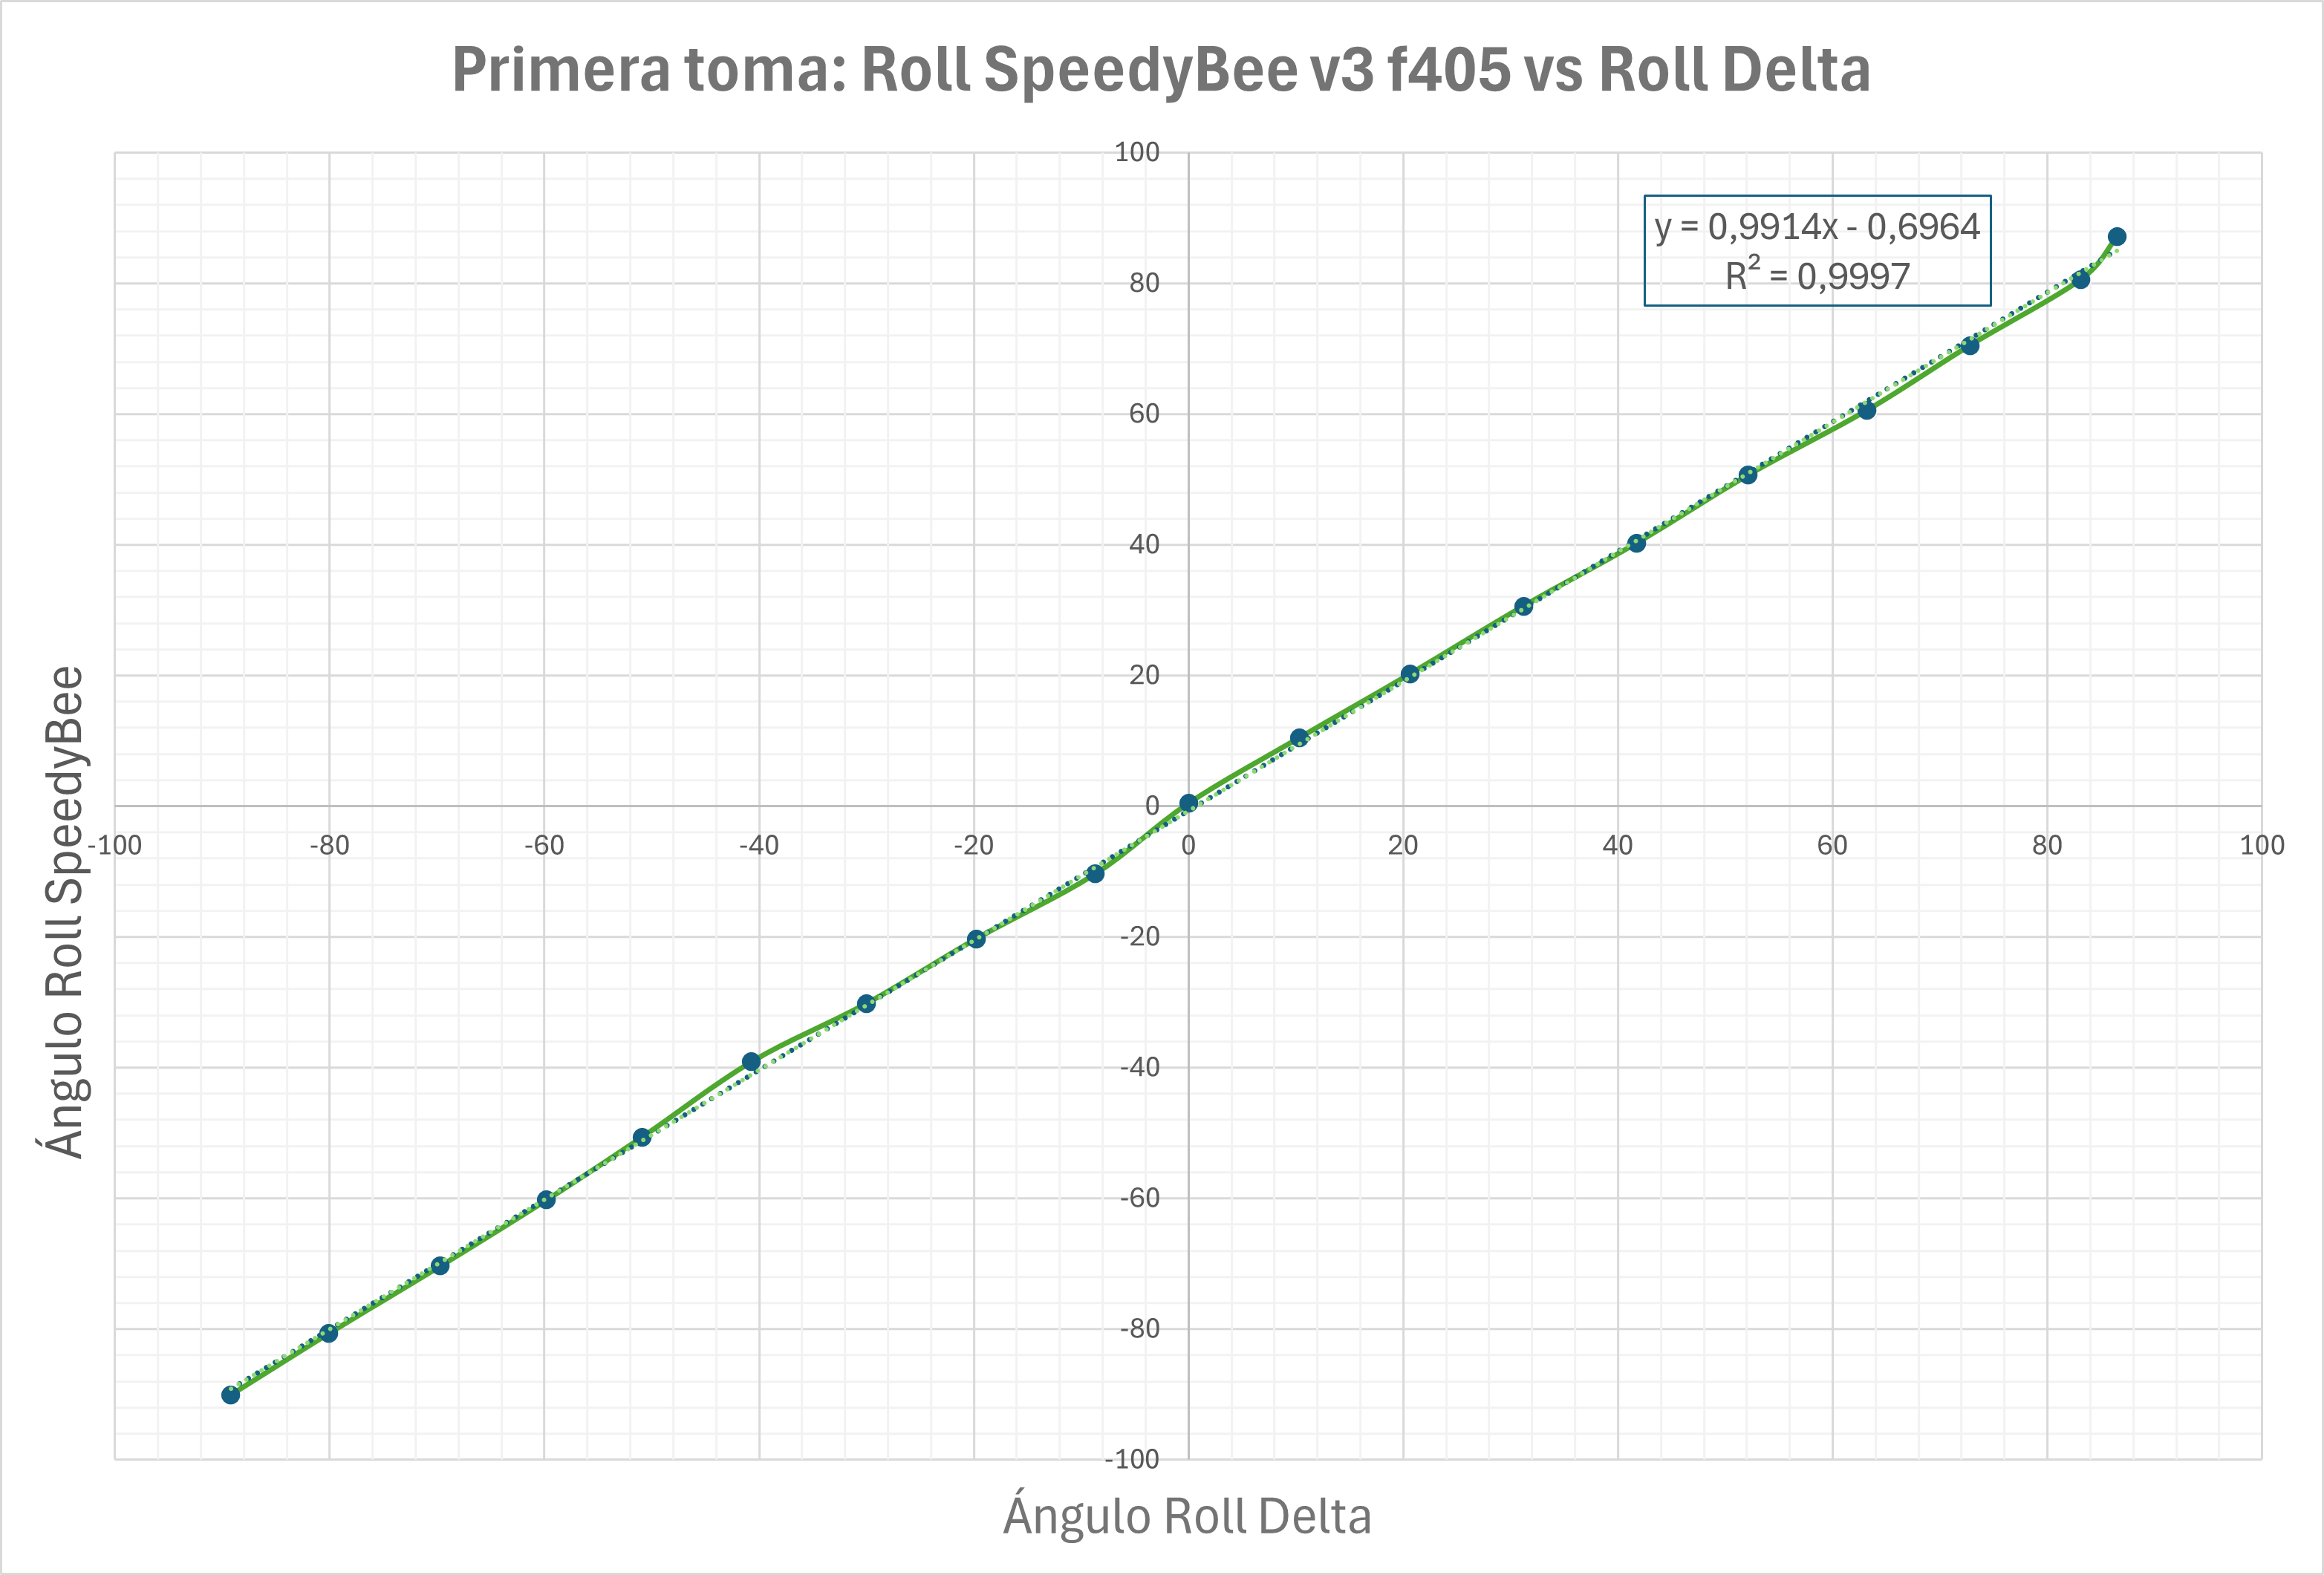
\includegraphics[width=5.5 in]{Imagenes/Pruebas/roll_1_compare.png}
                \caption{Comparación de ángulo Roll entre controladores Delta y SpeedyBee V3 F405 en la primera toma de datos }
                \label{fig:comparacionRoll}
            \end{figure}

            \begin{figure}[H]
                \centering
                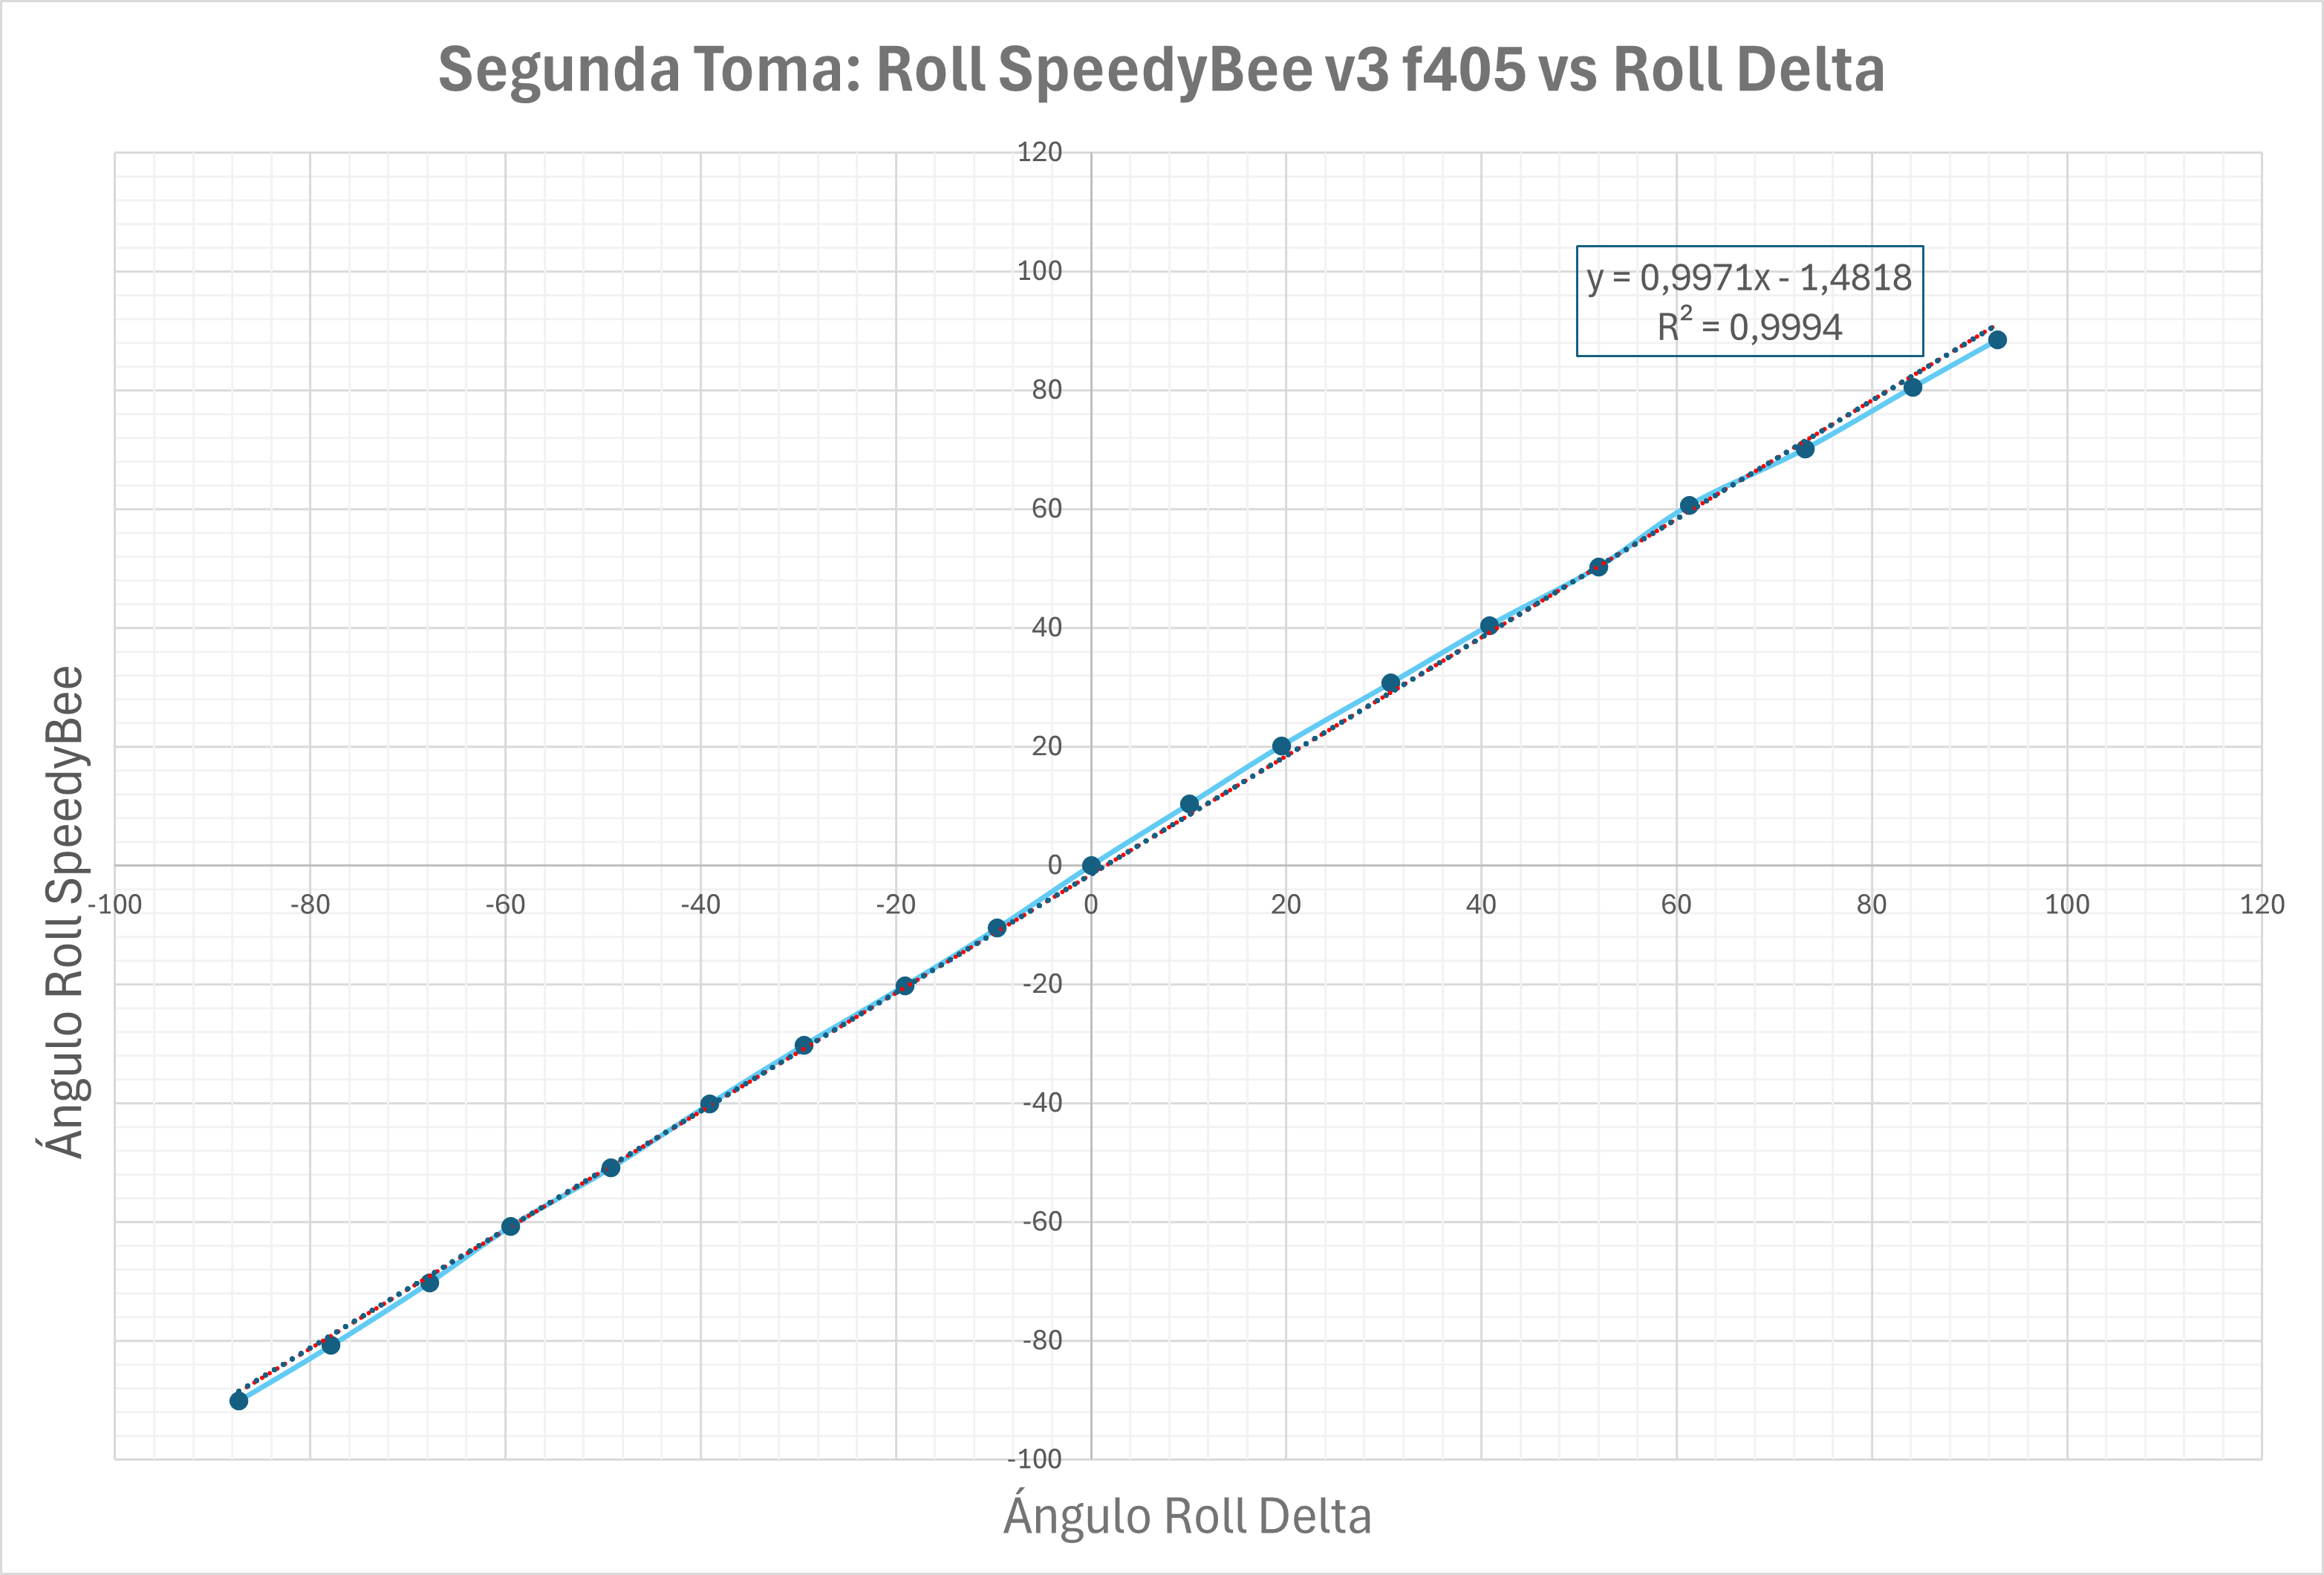
\includegraphics[width=5.5 in]{Imagenes/Pruebas/roll_2_compare.png}
                \caption{Comparación de Roll entre controladores Delta y SpeedyBee V3 F405 en la segunda toma de datos }
                \label{fig:comparacionRoll}
            \end{figure}


        \subsubsection{Comparación de Pitch}
            De manera similar, los gráficos de la Figura \ref{fig:comparacionPitch1} presentan la comparación de los ángulos de Pitch. Aquí también se evidencia que ambos controladores tienen un comportamiento muy parecido. Las diferencias entre los valores son mínimas y generalmente se mantienen dentro de un margen de error aceptable.


            \begin{figure}[H]
                \centering
                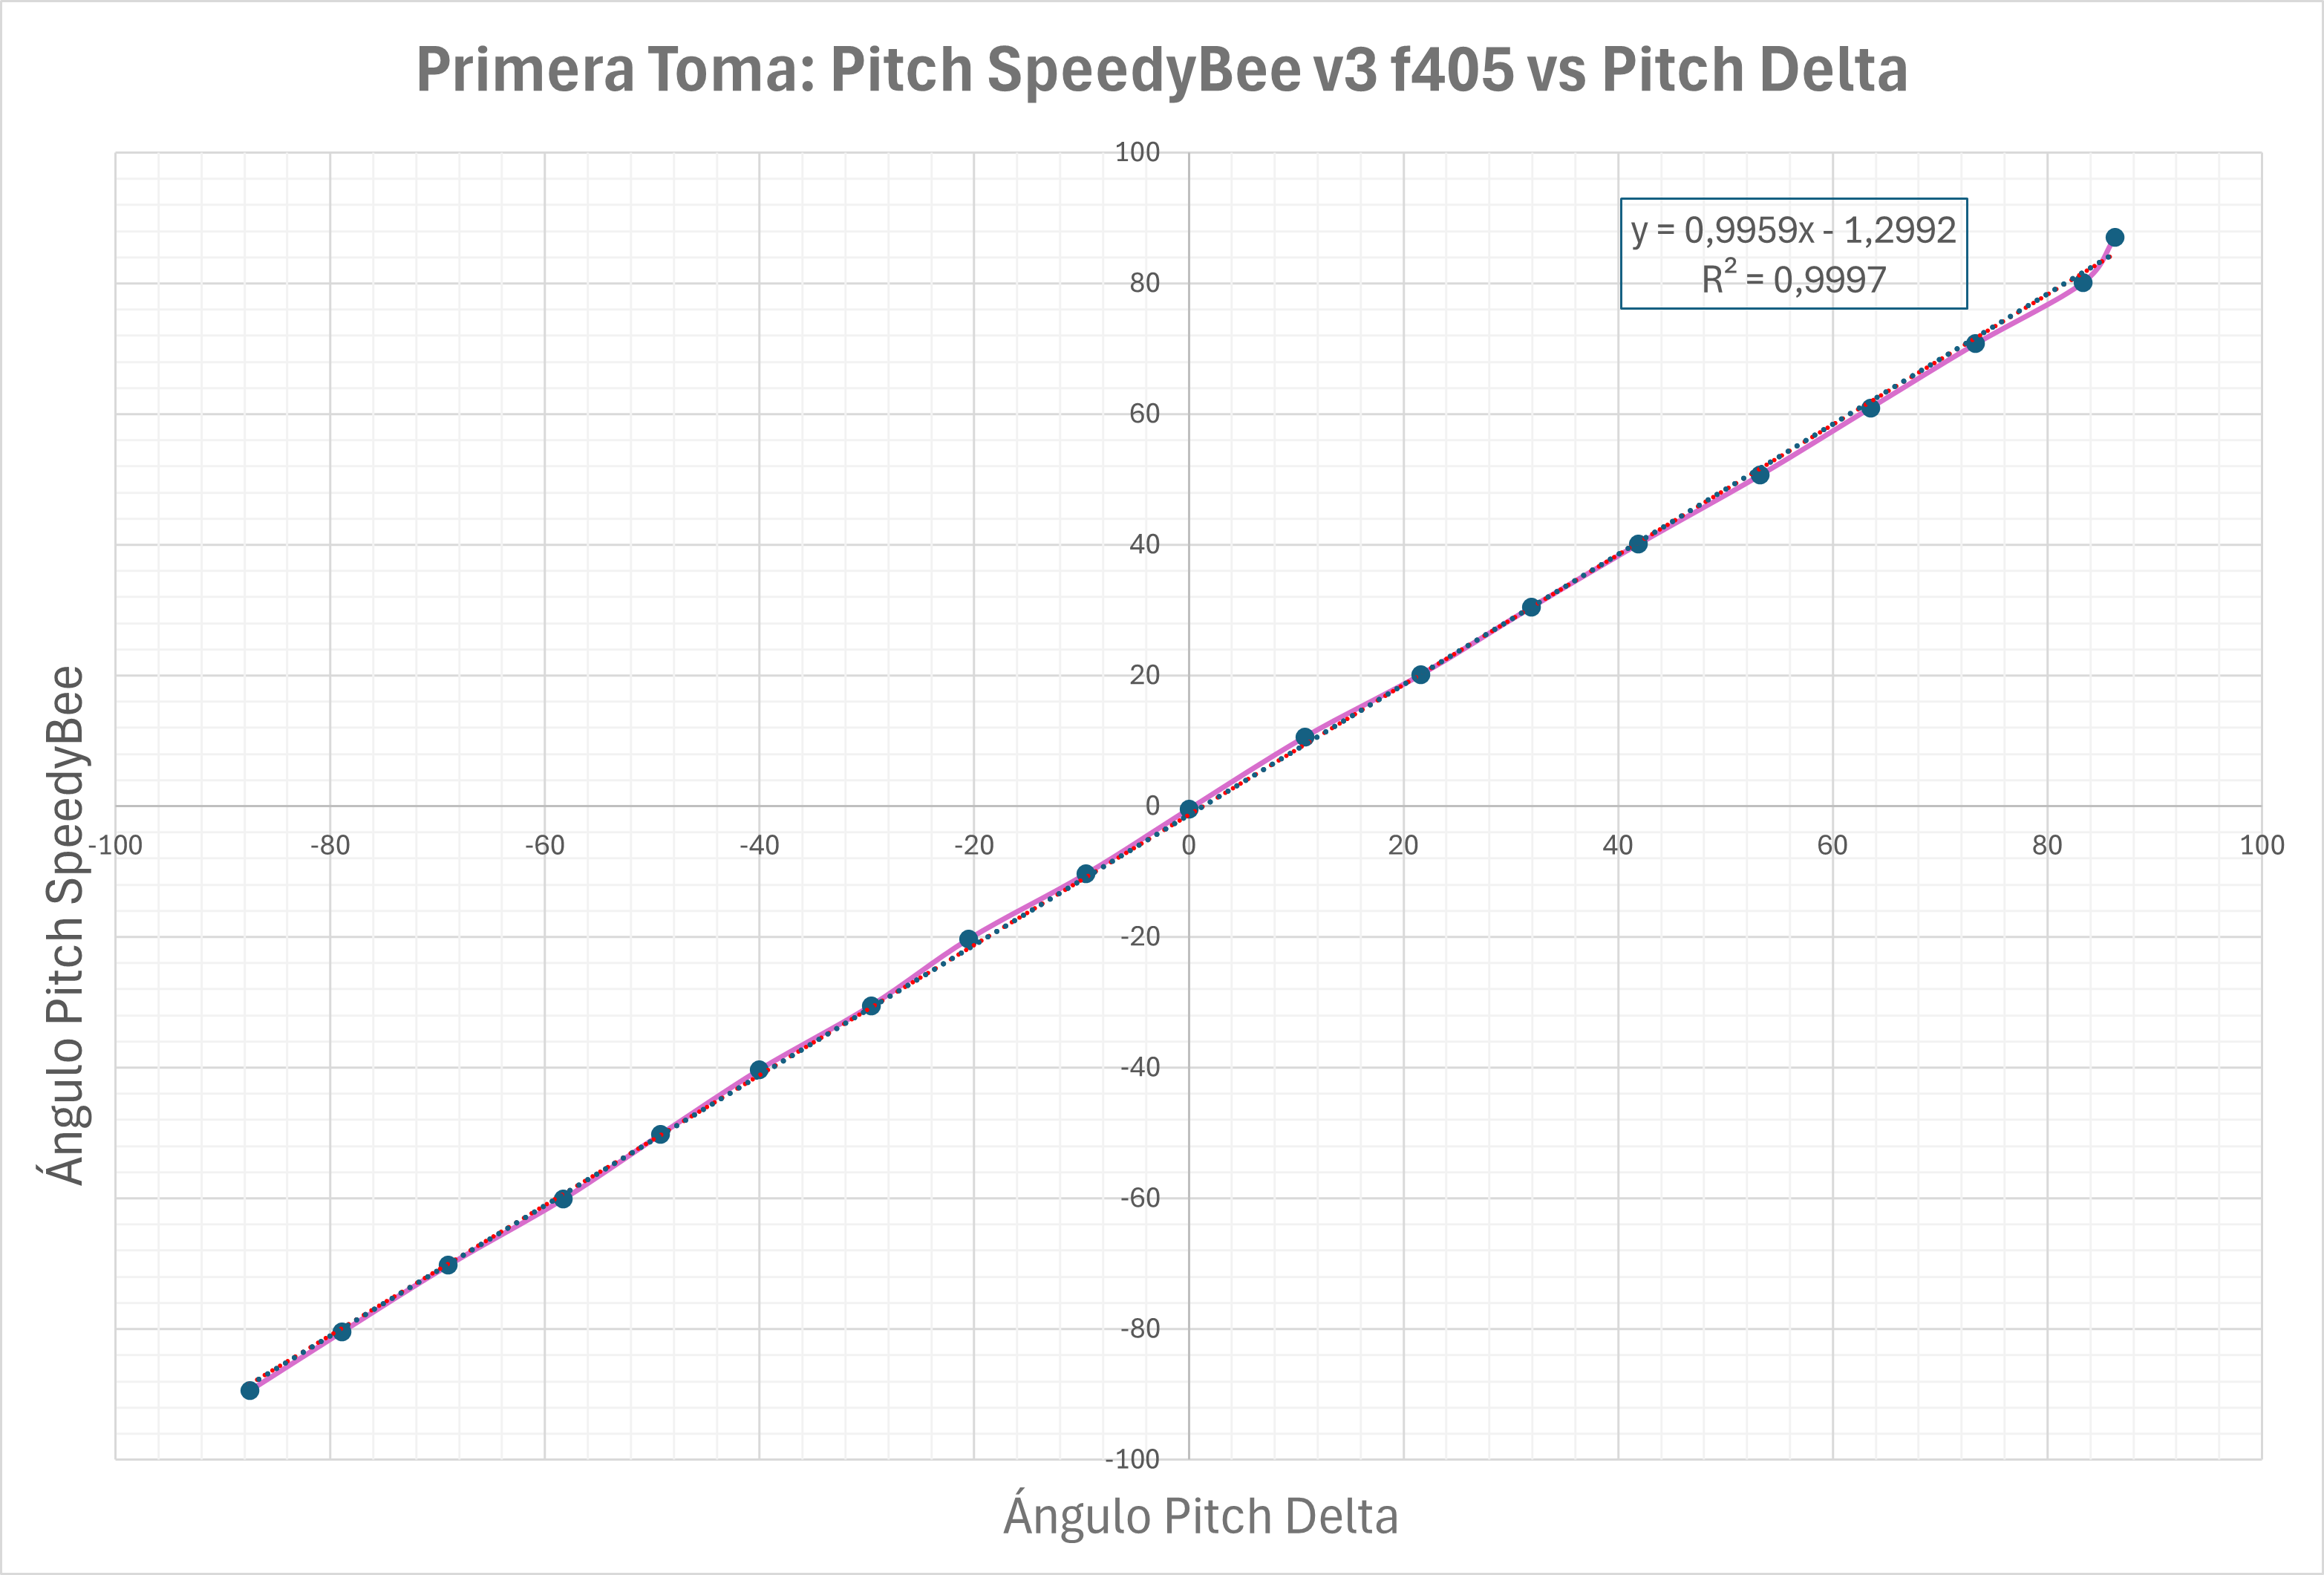
\includegraphics[width=5.5 in]{Imagenes/Pruebas/pitch_1_compare.png}
                \caption{Comparación de Pitch entre controladores Delta y SpeedyBee V3 F405 en la primera toma de datos }
                \label{fig:comparacionPitch1}
            \end{figure}

            \begin{figure}[H]
                \centering
                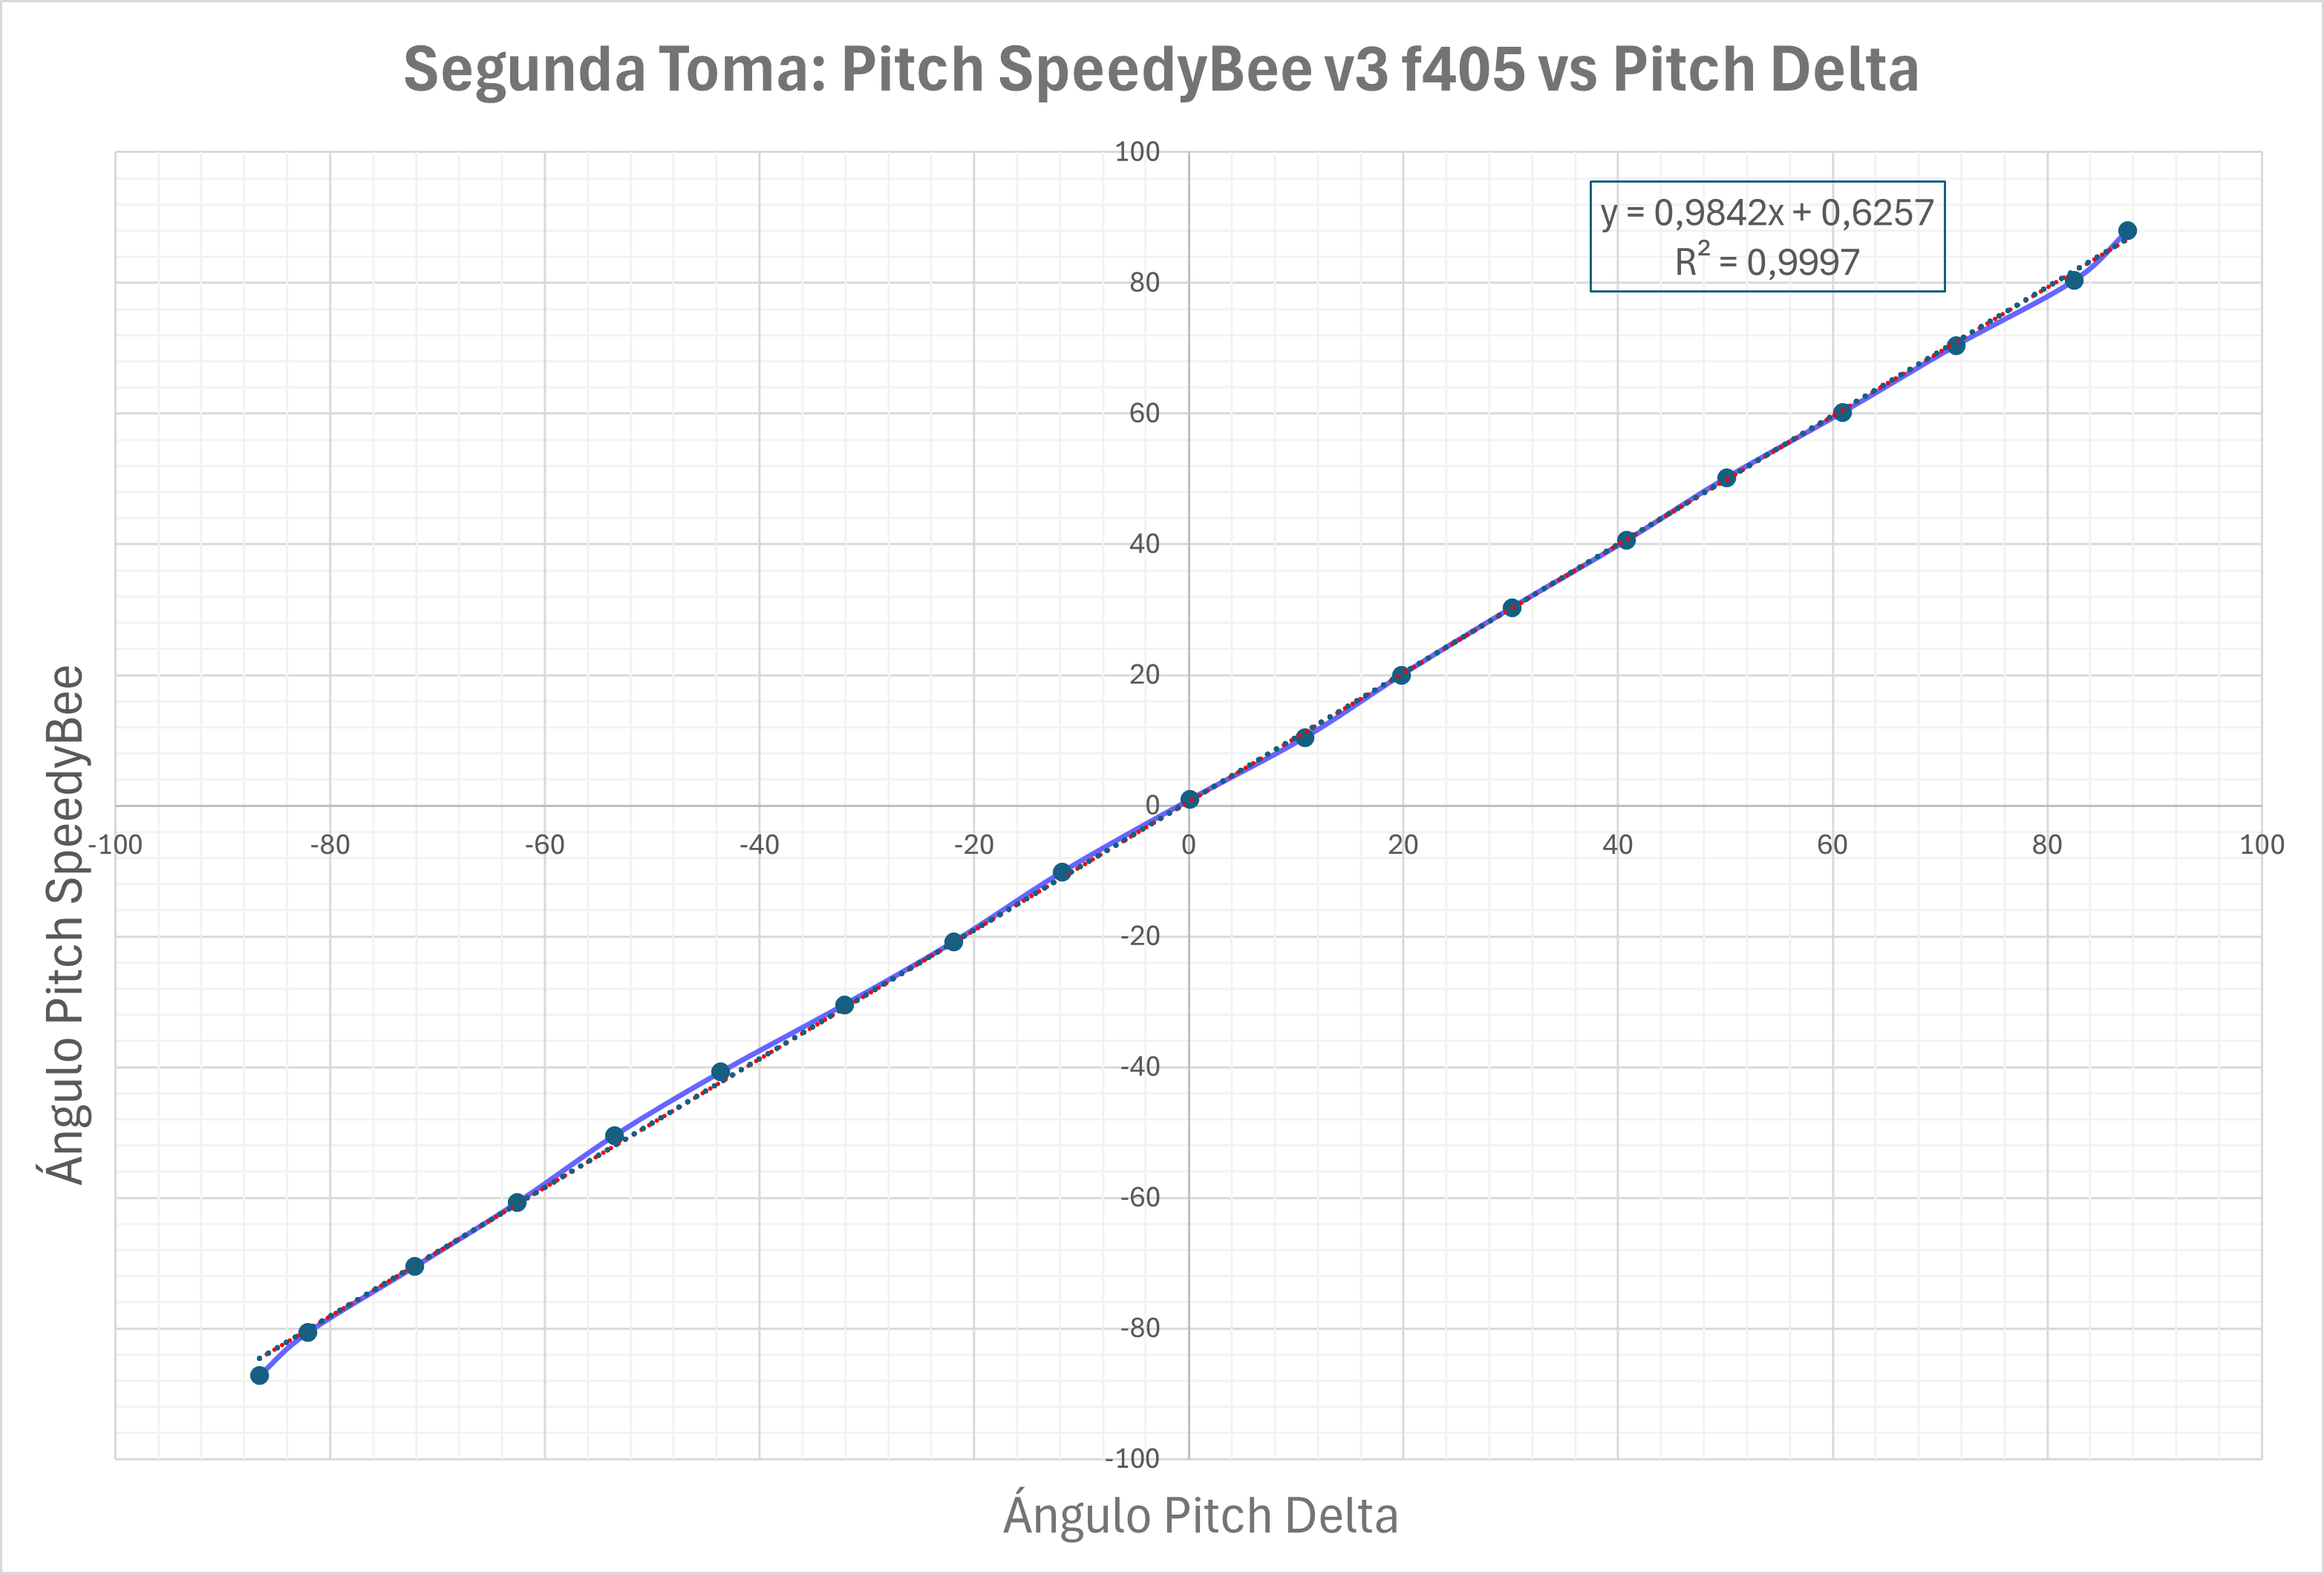
\includegraphics[width=5.5 in]{Imagenes/Pruebas/pitch_2_compare.png}
                \caption{Comparación de Roll entre controladores Delta y SpeedyBee V3 F405 en la segunda toma de datos }
                \label{fig:comparacionPitch2}
            \end{figure}


    \subsection{Pruebas de Variación de Altura con el Barómetro BMP280}

        Para evaluar el desempeño del sensor barométrico BMP280 en la medición de la altura, se realizó una prueba en el Edificio Mario Laserna. Durante esta prueba, se utilizó un ascensor para cambiar de piso en diferentes niveles del edificio. La prueba se inició en el nivel S2 y se ascendió hasta el piso 8. Finalmente, se descendió al nivel inicial y se capturaron los datos correspondientes a la variación de altura.

        \subsubsection{Procedimiento de la Prueba}

            \begin{enumerate}
                \item \textbf{Inicio en el Nivel S2}: La prueba comenzó en el nivel subterráneo 2 del edificio.
                \item \textbf{Ascenso al Piso 8}: Se utilizó el ascensor para ascender secuencialmente desde el nivel S2 hasta el piso 8, realizando paradas en cada piso para registrar los datos de altura.
                \item \textbf{Descenso al Nivel Inicial}: Posteriormente, se descendió de nuevo hasta el nivel S2, registrando los datos durante todo el recorrido.
            \end{enumerate}

        \subsubsection{Resultados}

            La figura adjunta muestra los resultados obtenidos de la prueba de variación de altura. Se puede observar cómo la altura medida por el BMP280 cambia a medida que el sensor se mueve a diferentes niveles del edificio. Los datos capturados reflejan un aumento progresivo de la altura durante el ascenso y una disminución correspondiente durante el descenso.

            \begin{figure}[H]
                \centering
                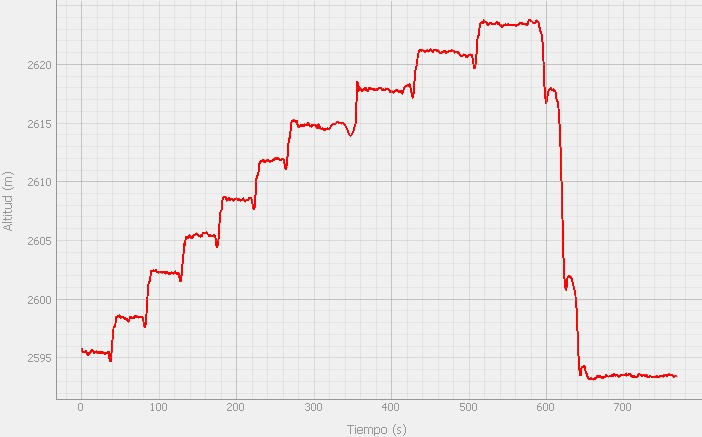
\includegraphics[width=0.8\textwidth]{Imagenes/Pruebas/altura.jpg}
                \caption{Variación de altura medida por el BMP280 durante el ascenso y descenso en el Edificio Mario Laserna.}
                \label{fig:variacion_altura}
            \end{figure}

        \subsubsection{Análisis de las Alturas del Edificio}

            La prueba de variación de altura realizada en el Edificio Mario Laserna nos permitió obtener datos precisos sobre la altitud a diferentes niveles del edificio. Según los datos registrados, la altura en el nivel S2 era de aproximadamente 2595 metros sobre el nivel del mar (msnm), mientras que en el piso 8 la altura era de aproximadamente 2625 metros msnm.

            Para calcular la diferencia de altura entre estos dos niveles, se realiza la siguiente operación:

            \[
            \text{Diferencia de altura} = 2625 \, \text{msnm} - 2595 \, \text{msnm} = 30 \, \text{metros}
            \]

            Por lo tanto, la altura total del edificio, desde el nivel S2 hasta el piso 8, es de 30 metros.

            Estos resultados demuestran la capacidad del sensor BMP280 para medir con precisión las variaciones de altura en un entorno controlado como el de un edificio de varios pisos.



    \subsection{Pruebas de GPS}
        Se realizó una prueba de GPS en el espacio abierto conocido como \textbf{El Bobo} en la Universidad de los Andes. Durante esta prueba, los datos de ubicación fueron almacenados en la tarjeta SD del dispositivo para su posterior análisis y ploteo en un mapa. Tal y como se muestra en la imagen adjunta, se realizó un desplazamiento en forma de bucle para verificar la precisión del GPS.

        El recorrido se realizó alrededor de la zona verde, registrando puntos de ubicación en intervalos regulares. Los datos capturados fueron luego representados en un mapa, mostrando el trayecto seguido. Esta prueba permitió evaluar la precisión del GPS en un entorno controlado y abierto, confirmando su capacidad para rastrear movimientos en tiempo real y proporcionar datos de ubicación precisos.

        \begin{figure}[H]
        \centering
        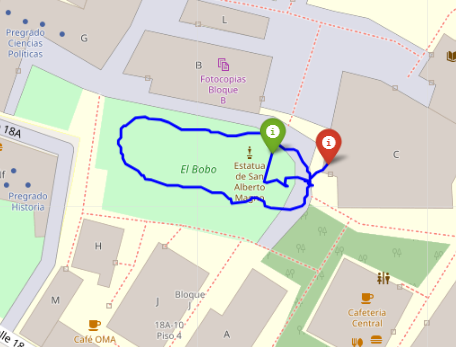
\includegraphics[width=0.8\textwidth]{Imagenes/Pruebas/gps.png}
        \caption{Recorrido de prueba de GPS en \textbf{El Bobo}, Universidad de los Andes.}
        \label{fig
        }
        \end{figure}